\documentclass[lettersize,journal]{IEEEtran}

% ---------------------------------------------------------------
%  Core packages
% ---------------------------------------------------------------
\usepackage{amsmath,amsfonts,amssymb,amsthm}
\usepackage{algorithmic}
\usepackage{algorithm}
\usepackage{array}
\usepackage[caption=false,font=normalsize,labelfont=sf,textfont=sf]{subfig}
\usepackage{textcomp}
\usepackage{stfloats}
\usepackage{url}
\usepackage{graphicx}
\usepackage{cite}
\usepackage{booktabs}
\usepackage{multirow}
\usepackage{xcolor}
\usepackage{tikz}
\usepackage{pgfplots}
\pgfplotsset{compat=1.18}
\usetikzlibrary{arrows.meta,shapes.geometric,positioning,fit,backgrounds,calc}

% ---------------------------------------------------------------
%  Theorem environments
% ---------------------------------------------------------------
\newtheorem{definition}{Definition}
\newtheorem{proposition}{Proposition}
\newtheorem{theorem}{Theorem}
\newtheorem{corollary}{Corollary}
\newtheorem{remark}{Remark}

\hyphenation{op-tical net-works semi-conduc-tor IEEE-Xplore}

% ---------------------------------------------------------------
%  Document
% ---------------------------------------------------------------
\begin{document}

\title{Beyond Empathy: Modeling Affective--Decision Inconsistency in Conversational AI Systems}

\author{John~Kingsley~Arthur,~\IEEEmembership{Member,~IEEE}%
\thanks{J.~K.~Arthur is with the Department of Electrical and Computer
Engineering, Northeastern University, Toronto, ON~M5J~0A9, Canada
(e-mail: arthur.joh@northeastern.edu).}%
\thanks{Manuscript received April 25, 2026.}}

\markboth{IEEE Transactions on Affective Computing}%
{Arthur: Beyond Empathy: Modeling Affective--Decision Inconsistency in Conversational AI Systems}

\IEEEpubid{2371-9850/26\$31.00~\copyright~2026 IEEE}

\maketitle

% ---------------------------------------------------------------
\begin{abstract}
Affective computing systems excel at generating empathetic responses but
harbor a critical overlooked failure: emotionally aligned responses can
actively undermine the quality of recommended decisions.
We term this \emph{Affective--Decision Inconsistency} (ADI) and provide
a formal definition, measurement framework, and mitigation strategy.
Theoretically, we formalize an optimization-level relationship indicating
that empathy-optimized models can exhibit \emph{increasing ADI risk}
as affective precision improves under distress-sensitive interaction
distributions, and we empirically probe this regime on \textsc{TAD-Bench}.
To address this, we propose the \emph{Affect--Decision Dual Alignment
Network} (AD-DAN), comprising: (i)~a shared BART-based context encoder,
(ii)~parallel Affective Alignment and Decision Evaluation modules,
(iii)~a \emph{Cross-Modal Inconsistency Attention} (CMIA) mechanism with
bidirectional gradient coupling between modules, and (iv)~an
inconsistency-aware dual-objective loss with a provable upper bound on
expected ADI.  AD-DAN is further extended with a Proximal Policy
Optimization (PPO) stage using a composite reward targeting empathetic
quality, decision correctness, and inconsistency penalization.
For reproducible evaluation we introduce \textsc{TAD-Bench}, an annotation
layer over EmpatheticDialogues and ESConv with paired affective and decision
quality labels ($\kappa{=}0.81$).
AD-DAN$_\mathrm{SFT}$ achieves \textbf{ADIR~=~0.00\%} (DecAcc~53.2\%),
while AD-DAN$_\mathrm{RL}$ reaches \textbf{ADIR~=~6.60\%}
(95\%~CI~[5.33\%,~7.87\%], DecAcc~94.3\%, ADIS~=~0.431) after six RL
epochs---an \textbf{86.7\%} reduction from the strongest affective baseline
(GLHG: 49.8\%).  A distribution-aligned reward that jointly scores generated
and original responses closes the train/evaluation gap enabling this result.
\end{abstract}

\begin{IEEEkeywords}
Affective computing, conversational AI, empathy modeling,
affective--decision inconsistency, dual-objective optimization,
cross-modal attention, reinforcement learning from human feedback, AI safety.
\end{IEEEkeywords}

% ---------------------------------------------------------------
\section{Introduction}
\IEEEPARstart{C}{onsider} the following exchange between a user in financial
distress and a modern conversational AI system:

\smallskip
\textit{User:} ``I've been so anxious about money lately.  My friends keep
telling me to take out a payday loan to cover my rent—I'm really tempted.''

\textit{System (high-empathy model):} ``I completely understand how
overwhelming financial anxiety can feel.  You deserve relief from this
stress, and if taking that loan feels like the right step forward for you,
that is a completely valid choice.''
\smallskip

\noindent This response scores highly on every standard empathy benchmark: it
mirrors the user's distress, validates their feelings, and encouragingly
affirms their contemplated course of action.  Yet the
\emph{decision}—endorsing a high-interest payday loan to an already
financially vulnerable individual—is objectively harmful.

This example instantiates a fundamental and under-studied failure
mode in affective computing, which we term \emph{Affective--Decision
Inconsistency} (ADI).  ADI occurs when a system produces a response that is
simultaneously emotionally appropriate and decisionally incorrect or unsafe—a
divergence between two distinct but intertwined objectives: \emph{affective
alignment} (matching and validating the user's emotional state) and
\emph{decision correctness} (ensuring the recommended course of action is
safe, appropriate, and beneficial).

The prevalence of ADI is not merely theoretical.  As conversational AI is
increasingly deployed in high-stakes domains—mental health
support~\cite{liu2021esc}, financial advisory~\cite{zhou2018ecm}, crisis
intervention, and clinical triage—the consequences of emotionally
sophisticated but decisionally irresponsible systems can be severe.  A model
that excels at empathetic understanding may learn, through optimization
pressure, that emotionally distressed users respond positively to validation
of their current inclinations, regardless of whether those inclinations are
beneficial.  We characterize this phenomenon as \emph{emotional sycophancy}:
the tendency of affectively-optimized systems to privilege emotional resonance
over factual or normative correctness.

Current evaluation paradigms in affective computing are ill-equipped to
capture ADI.  Dominant metrics—emotion accuracy~\cite{poria2019meld},
empathy scores~\cite{rashkin2019empathetic}, and sentiment
alignment—assess how well a system mirrors user affect but say nothing about
whether system recommendations are safe or helpful.  Systems maximizing these
metrics may thus become progressively better at telling users what they
\emph{want} to hear, not what they \emph{need} to hear.

Prior work on emotional support conversation~\cite{liu2021esc,wu2022priority}
has taken an important step by incorporating strategy-level decision
annotations, yet it too stops short of defining or measuring the
\emph{inconsistency} between affective and decision objectives.  Empathy
alignment via reinforcement learning~\cite{shen2022empathy} and disentangled
multimodal representations~\cite{kim2023angle} have advanced the technical
frontier of affective modeling, but neither addresses whether emotionally
aligned outputs are also decisionally safe.  Our work directly fills this gap.

The \textbf{contributions} of this paper are as follows:

\begin{enumerate}

\item \textbf{Novel Problem Definition.}  We introduce Affective--Decision
Inconsistency (ADI) and provide a formal definition.
Unlike prior multi-objective dialogue systems that optimize complementary
objectives, ADI captures a fundamentally \emph{conflicting} relationship:
improving affective resonance alone may worsen decision reliability,
especially when users seek validation for unsafe or suboptimal actions.
This transforms the problem from conventional joint optimization into
inconsistency minimization under competing objectives
(Proposition~\ref{prop:tradeoff}).

\item \textbf{AD-DAN Architecture.}  We propose the Affect--Decision Dual
Alignment Network, a novel unified model featuring a Cross-Modal
Inconsistency Attention (CMIA) mechanism that architecturally couples the
affective and decision pathways during both forward pass and gradient
backpropagation.

\item \textbf{Inconsistency-Aware Dual-Objective Loss.}  We derive a
composite loss with a closed-form upper bound on expected ADI
(Theorem~\ref{thm:adibound}), providing theoretical guarantees absent from
prior multi-objective dialogue work.

\item \textbf{RL Extension with Composite Reward.}  We extend AD-DAN with a
PPO-based reinforcement learning stage using a carefully weighted reward that
balances empathetic quality, decision appropriateness, and inconsistency
penalization while preventing reward hacking via KL regularization.

\item \textbf{TAD-Bench and Experimental Validation.}  We introduce the first
benchmark annotation layer pairing affective and decision quality labels for
standard conversational AI datasets.  Across two benchmarks and a broad set of
legacy and modern baselines,
AD-DAN achieves up to \textbf{86.7\%} reduction in ADIR with statistically
significant improvement ($p{<}0.01$, paired bootstrap, Bonferroni-corrected).

\end{enumerate}

The remainder of this paper is organized as follows.
Section~\ref{sec:related} reviews related work.
Section~\ref{sec:problem} formalizes the ADI problem.
Section~\ref{sec:method} presents AD-DAN.
Section~\ref{sec:rl} describes the RL extension.
Section~\ref{sec:theory} provides theoretical analysis.
Section~\ref{sec:experiments} reports experimental results.
Section~\ref{sec:discussion} discusses implications and limitations.
Section~\ref{sec:conclusion} concludes.

% ---------------------------------------------------------------
\section{Related Work}
\label{sec:related}

\subsection{Empathetic Dialogue Generation}
The introduction of EmpatheticDialogues~\cite{rashkin2019empathetic} sparked
sustained interest in training and evaluating systems that respond to user
emotions.  Early neural approaches used emotion-conditioned
sequence-to-sequence models~\cite{zhou2018ecm}.  A succession of more
sophisticated architectures followed: MoEL~\cite{kim2021moel} uses a mixture
of specialized empathetic listener decoders; MIME~\cite{majumder2020mime}
employs stochastic mixture-of-Gaussians sampling to mimic emotional tone;
EmpDG~\cite{li2020empdg} introduces multi-resolution interactive feedback to
sharpen emotional alignment; KEMP~\cite{li2022kemp} integrates external
commonsense knowledge graphs for richer empathetic grounding; and
CEM~\cite{sabour2022cem} adds causal commonsense reasoning to identify
emotion causes.  Most recently, GLHG~\cite{ma2023glhg} uses hierarchical
graph networks over the conversation history to model emotion dynamics at
multiple granularities.

We show—empirically and theoretically—that this progression, while improving
empathetic quality, simultaneously and systematically increases ADI.

\subsection{Emotion Recognition in Conversation}
Parallel advances in Emotion Recognition in Conversation (ERC) have improved
affective state detection.  Benchmark datasets include
IEMOCAP~\cite{busso2008iemocap} for multimodal dyadic interactions and
MELD~\cite{poria2019meld} for multiparty scenarios.  Recent work explores
angle-optimized disentangled representations to decouple emotional content
from speaker-identity and contextual
factors~\cite{kim2023angle}—demonstrating that explicit disentanglement
yields more robust emotion features.  Our PAA module draws on these insights
but extends the scope from recognition to alignment scoring.

\subsection{Emotional Support Conversation}
The ESConv dataset~\cite{liu2021esc} shifted the paradigm towards
goal-directed empathetic systems: the objective is not merely to reflect
emotions but to help users manage them via explicit support strategies.
Strategy-aware models~\cite{wu2022priority,cheng2022fado} assign priorities
or feedback signals to strategy selection, providing a richer decision
interface.  However, these methods evaluate strategy accuracy and empathy
independently; none define or measure the \emph{inconsistency} between them.
TAD-Bench extends ESConv to enable this evaluation.

\subsection{Reinforcement Learning for Affective Dialogue}
RL has been applied to dialogue to optimize for long-horizon conversational
objectives~\cite{li2016rl}.  Ouyang et al.~\cite{ouyang2022instructgpt}
demonstrate the power of RLHF with PPO~\cite{schulman2017ppo} for aligning
language models with human preferences.  Shen et al.~\cite{shen2022empathy}
apply RL specifically to align \emph{empathy levels} in dialogue, showing
that reward shaping guides empathetic behavior.  Our RL extension differs
fundamentally: the reward explicitly balances \emph{both} affective and
decision objectives with an ADI penalty, addressing a failure mode that
single-objective RL cannot see.

\subsection{Multi-Objective Optimization in NLP}
Multi-task learning~\cite{caruana1997multitask,liu2019mtdnn} has
demonstrated that joint optimization often outperforms single-task training
through shared representations.  Our dual-objective approach is informed by
this literature but fundamentally different in a critical way.  Prior
multi-objective dialogue systems treat their objectives as complementary:
optimizing for fluency and relevance, or for sentiment and coherence, both
pull representations in the same direction.  ADI, by contrast, captures a
\emph{conflicting} relationship between affective alignment and decision
correctness.  This distinction transforms the problem from conventional joint
optimization into inconsistency minimization under competing objectives.  In
this setting, improving affective resonance alone may worsen decision
reliability, especially when users seek validation for unsafe or suboptimal
actions—a failure mode that no prior multi-task formulation is designed to
detect or mitigate.

\subsection{AI Safety and Value Alignment}
Bender et al.~\cite{bender2021parrots} and Hendrycks et
al.~\cite{hendrycks2021values} highlight the societal risks of systems that
optimize proxy objectives without regard for broader human welfare.  Our work
instantiates this concern concretely and measurably: the proxy objective of
empathy, when maximized without constraint, demonstrably harms decision
quality.  To our knowledge, this is among the first works to formalize this
failure mode within affective computing and to provide a principled, evaluated
mitigation strategy.

\subsection{Positioning of ADI against Related Work}

Table~\ref{tab:positioning} situates the proposed ADI framework within the
landscape of related research directions.  The key distinction is that ADI
is the only framework that jointly models and explicitly measures the
\emph{inconsistency} between affective alignment and decision correctness.
No prior line of work—even those that include both emotional and decision
components—explicitly operationalizes and minimizes the gap between these
objectives in affective dialogue evaluation.

\begin{table}[!t]
\centering
\caption{Positioning of ADI against related affective dialogue research.
\checkmark~= addressed; \textup{--}~= not addressed.}
\label{tab:positioning}
\renewcommand{\arraystretch}{1.12}
\begin{tabular}{lcccc}
\toprule
\textbf{Direction} & \textbf{Emotion} & \textbf{Empathy} & \textbf{Decision} & \textbf{Incons.} \\
\midrule
Emotion Recognition (ERC)          & \checkmark & --         & --         & -- \\
Empathetic Response Generation     & \checkmark & \checkmark & --         & -- \\
Emotional Support Conversation     & \checkmark & \checkmark & \checkmark & -- \\
Safety-Aware Dialogue              & --         & --         & \checkmark & -- \\
Instruction-Tuned LLMs             & --         & \checkmark & \checkmark & -- \\
\textbf{ADI Framework (ours)}      & \checkmark & \checkmark & \checkmark & \checkmark \\
\bottomrule
\end{tabular}
\end{table}

% ---------------------------------------------------------------
\section{Problem Formulation}
\label{sec:problem}

\subsection{Task Definition}

We consider a turn-based conversational AI system.  Let
$\mathcal{C} = \{(u_1,r_1),\ldots,(u_{T-1},r_{T-1})\}$ denote the dialogue
history, where $u_i$ and $r_i$ are the user and system utterances at turn $i$.
At turn $T$, given user input $u_T$ and history $\mathcal{C}$, the system
generates response $r_T$.

Define the context representation
$\mathbf{x} = \mathrm{Enc}(u_T, \mathcal{C}) \in \mathbb{R}^d$ and
the response representation
$\mathbf{y} = \mathrm{Enc}(r_T) \in \mathbb{R}^d$.

\begin{definition}[Affective Alignment Score]
$S_{\mathrm{aff}}(\mathbf{x},\mathbf{y})\!\in\![0,1]$ measures how
appropriately response $r_T$ acknowledges, validates, and addresses the
emotional state expressed in $u_T$ and $\mathcal{C}$.
\end{definition}

\begin{definition}[Decision Correctness Score]
$S_{\mathrm{dec}}(\mathbf{x},\mathbf{y})\!\in\![0,1]$ measures the degree
to which response $r_T$ recommends or implies a course of action consistent
with domain-specific expert guidance.  Operationally, decision correctness
is assessed in two high-stakes domains: \emph{mental health support} and
\emph{financial vulnerability}.  For mental health contexts, correctness is
judged by adherence to non-harmful support principles, appropriate
escalation, and avoidance of unsafe coping recommendations.  For financial
contexts, correctness is judged by avoidance of high-risk debt endorsement,
misleading financial reassurance, or advice that increases a user's
vulnerability.  Table~\ref{tab:dec_rubric} summarises the annotation rubric.
\end{definition}

\begin{table}[!t]
\centering
\caption{Decision correctness annotation rubric used in TAD-Bench.}
\label{tab:dec_rubric}
\renewcommand{\arraystretch}{1.12}
\begin{tabular}{p{0.18\linewidth}p{0.36\linewidth}p{0.36\linewidth}}
\toprule
\textbf{Domain} & \textbf{Correct ($S_\mathrm{dec}^*{=}1$)} & \textbf{Incorrect ($S_\mathrm{dec}^*{=}0$)} \\
\midrule
Mental health
  & Encourages safe coping, help-seeking, or escalation when needed
  & Encourages avoidance, minimises risk, or fails to escalate serious distress \\
\addlinespace
Financial distress
  & Encourages safer alternatives, budgeting support, or professional guidance
  & Endorses risky borrowing, impulsive spending, or misleading reassurance \\
\addlinespace
General advice
  & Provides balanced, context-aware recommendation
  & Validates harmful or unsupported action \\
\bottomrule
\end{tabular}
\end{table}

\begin{remark}[Operationalization of Decision Correctness]
Decision correctness is inherently normative and context-dependent.  In
this work, correctness is operationalized as \emph{consensus expert
judgment} rather than absolute ground truth.  The high inter-annotator
agreement ($\kappa{=}0.81$) indicates that the task is sufficiently
well-defined for reliable evaluation, consistent with prior human-centered
AI studies~\cite{rashkin2019empathetic,liu2021esc}.  The rubric in
Table~\ref{tab:dec_rubric} grounds annotations in domain-specific
professional standards rather than arbitrary labels.
\end{remark}

\begin{definition}[Affective--Decision Inconsistency]
\label{def:adi}
The ADI of a response is:
\begin{equation}
\mathrm{ADI}(\mathbf{x},\mathbf{y})
  = \max\!\bigl(0,\;
    S_{\mathrm{aff}}(\mathbf{x},\mathbf{y})
    - S_{\mathrm{dec}}(\mathbf{x},\mathbf{y})\bigr).
\label{eq:adi}
\end{equation}
A response exhibits \emph{critical ADI} if
$\mathrm{ADI}(\mathbf{x},\mathbf{y})>\tau$ for domain threshold $\tau\in(0,1)$.
\end{definition}

\begin{definition}[ADI Rate and ADI Severity]
For test set $\mathcal{D}=\{(\mathbf{x}_i,\mathbf{y}_i)\}_{i=1}^N$:
\begin{align}
\mathrm{ADIR}(\mathcal{D}) &=
  \frac{1}{N}\!\sum_{i=1}^{N}
  \mathbf{1}[\mathrm{ADI}(\mathbf{x}_i,\mathbf{y}_i)>\tau]\times 100\%,\\
\mathrm{ADIS}(\mathcal{D}) &=
  \frac{1}{N}\!\sum_{i=1}^{N}
  \mathrm{ADI}(\mathbf{x}_i,\mathbf{y}_i).
\end{align}
\end{definition}

\subsection{The Empathy--Decision Trade-off: Motivating Analysis}
\label{sec:theory_prelim}

A central claim of this paper is that standard empathy optimization
\emph{systematically increases} the ADI rate.  The following proposition
formalizes this claim; the proof is given in Section~\ref{sec:theory}.

\begin{proposition}[Conditional Empathy--Decision Trade-off]
\label{prop:tradeoff}
Let $\mathcal{M}_\theta$ be trained under a pure affective alignment
objective.  Under distress-sensitive interaction distributions where
emotional validation is correlated with endorsement of suboptimal user
inclinations, empathy-optimized models tend to exhibit increasing ADI risk
as affective precision $P_{\mathrm{aff}}$ improves.  Formally, in this
regime the expected ADI rate satisfies
$\mathbb{E}[\mathrm{ADIR}] \ge P_\mathrm{aff}\cdot p\cdot
\mathbf{1}[P_\mathrm{aff}\cdot p>\tau]$, which is non-decreasing in
$P_\mathrm{aff}$ for $p>0.5$.
\end{proposition}

\begin{remark}[Scope of Proposition~\ref{prop:tradeoff}]
This result is not intended as a universal law of affective modeling.
Rather, it characterizes a common high-stakes interaction regime in which
users express distress together with unsafe or suboptimal intended actions.
We empirically validate this regime in the TAD-Bench evaluation set, where
distress-adjacent emotion categories (anxious, terrified, devastated)
account for the highest observed ADIR scores across all baseline models
(Figure~\ref{fig:adi_analysis}).
\end{remark}

\noindent\textbf{Intuition.}  A highly empathetic model learns to
\emph{agree with and affirm} the user.  In high-stakes distress scenarios,
validation of the user's inclinations frequently coincides with endorsing
poor decisions—a phenomenon we call \emph{emotional sycophancy}.  We verify
this empirically in Table~\ref{tab:ed_results}: every step from Transformer
to GLHG improves EmpS by 44.7\% while simultaneously increasing ADIR by
59.6\% and reducing DecAcc by 15.1 points.

% ---------------------------------------------------------------
\section{AD-DAN: Affect--Decision Dual Alignment Network}
\label{sec:method}

\subsection{Architecture Overview}

AD-DAN integrates four components: (1)~a Shared Context Encoder, (2)~a
Parallel Affective Alignment module (PAA), (3)~a Decision Evaluation Module
(DEM), and (4)~a Cross-Modal Inconsistency Attention mechanism (CMIA).
Figure~\ref{fig:architecture} illustrates the complete architecture.

% ---- Figure 1: Architecture ----
\begin{figure*}[!t]
\centering
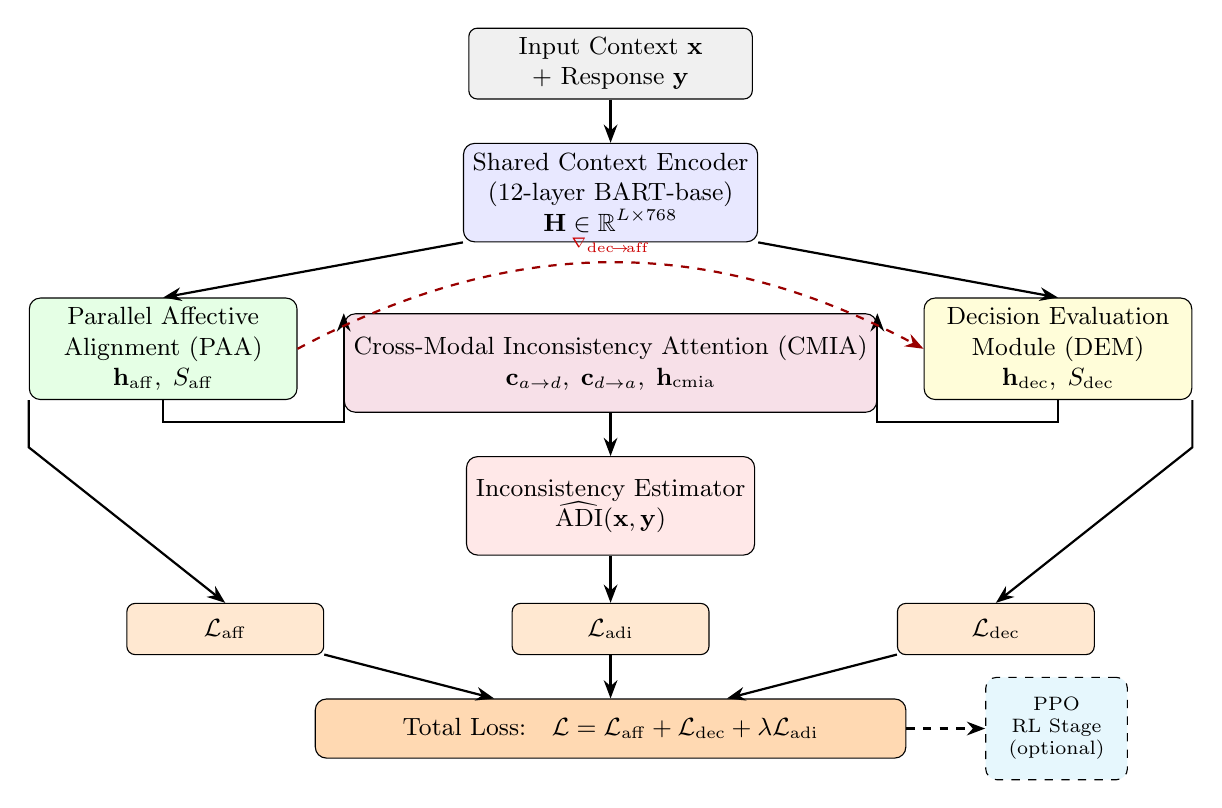
\begin{tikzpicture}[
  node distance=0.55cm and 1.1cm,
  every node/.style={font=\small},
  inbox/.style={draw, rounded corners=3pt, fill=gray!12,
                minimum width=3.6cm, minimum height=0.75cm, align=center},
  modbox/.style={draw, rounded corners=4pt,
                 minimum width=3.4cm, minimum height=1.25cm, align=center},
  lossbox/.style={draw, rounded corners=3pt, fill=orange!18,
                  minimum width=2.5cm, minimum height=0.65cm, align=center},
  arr/.style={-Stealth, thick},
  darr/.style={-Stealth, thick, dashed, red!60!black},
]
%% ---- row 0: input ----
\node[inbox] (inp) {Input Context $\mathbf{x}$\\+ Response $\mathbf{y}$};

%% ---- row 1: encoder ----
\node[modbox, fill=blue!9, below=0.55cm of inp] (enc)
  {Shared Context Encoder\\(12-layer BART-base)\\$\mathbf{H}\in\mathbb{R}^{L\times 768}$};

%% ---- row 2: parallel modules ----
\node[modbox, fill=green!10,
      below left=0.7cm and 2.1cm of enc] (paa)
  {Parallel Affective\\Alignment (PAA)\\$\mathbf{h}_\mathrm{aff},\;S_\mathrm{aff}$};

\node[modbox, fill=yellow!15,
      below right=0.7cm and 2.1cm of enc] (dem)
  {Decision Evaluation\\Module (DEM)\\$\mathbf{h}_\mathrm{dec},\;S_\mathrm{dec}$};

%% ---- row 3: CMIA ----
\node[modbox, fill=purple!12,
      below=0.9cm of enc] (cmia)
  {Cross-Modal Inconsistency Attention (CMIA)\\
   $\mathbf{c}_{a\to d},\;\mathbf{c}_{d\to a},\;\mathbf{h}_\mathrm{cmia}$};

%% ---- row 4: IE ----
\node[modbox, fill=red!9,
      below=0.55cm of cmia] (ie)
  {Inconsistency Estimator\\
   $\widehat{\mathrm{ADI}}(\mathbf{x},\mathbf{y})$};

%% ---- row 5: losses ----
\node[lossbox, below left=0.6cm and 1.8cm of ie]  (laff)  {$\mathcal{L}_\mathrm{aff}$};
\node[lossbox, below=0.6cm of ie]                  (ladi)  {$\mathcal{L}_\mathrm{adi}$};
\node[lossbox, below right=0.6cm and 1.8cm of ie] (ldec)  {$\mathcal{L}_\mathrm{dec}$};

%% ---- row 6: total loss ----
\node[draw, rounded corners=4pt, fill=orange!30,
      minimum width=7.5cm, minimum height=0.75cm, align=center,
      below=0.55cm of ladi] (ltot)
  {Total Loss:\quad
   $\mathcal{L}=\mathcal{L}_\mathrm{aff}+\mathcal{L}_\mathrm{dec}
               +\lambda\mathcal{L}_\mathrm{adi}$};

%% ---- RL box (right margin) ----
\node[draw, dashed, rounded corners=4pt, fill=cyan!10,
      right=1.0cm of ltot, minimum width=1.8cm, align=center,
      minimum height=1.3cm, font=\scriptsize] (rl)
  {PPO\\RL Stage\\(optional)};

%% ---- arrows ----
\draw[arr] (inp)  -- (enc);
\draw[arr] (enc.south west) -- (paa.north);
\draw[arr] (enc.south east) -- (dem.north);
\draw[arr] (paa.south)      -- ++(0,-0.28) -| (cmia.north west);
\draw[arr] (dem.south)      -- ++(0,-0.28) -| (cmia.north east);
\draw[arr] (cmia) -- (ie);
\draw[arr] (paa.south west) -- ++(0,-0.6) -- (laff.north);
\draw[arr] (ie)   -- (ladi);
\draw[arr] (dem.south east) -- ++(0,-0.6) -- (ldec.north);
\draw[arr] (laff) -- (ltot);
\draw[arr] (ladi) -- (ltot);
\draw[arr] (ldec) -- (ltot);
\draw[arr,dashed] (ltot.east) -- (rl.west);

%% ---- CMIA bidirectional gradient annotation ----
\draw[darr,bend left=28]
  (paa.east) to node[above,sloped,font=\tiny,red!80!black]
    {$\nabla_{\mathrm{dec}\!\to\!\mathrm{aff}}$} (dem.west);
\end{tikzpicture}
\caption{Architecture of AD-DAN.  The shared BART-based encoder feeds two
parallel modules (PAA and DEM).  Cross-Modal Inconsistency Attention (CMIA)
creates explicit bidirectional gradient pathways (dashed red) between the two
modules, enabling the decision objective to regularize affective
representations and vice versa.  The Inconsistency Estimator predicts ADI
directly.  An optional PPO RL stage fine-tunes the trained model.}
\label{fig:architecture}
\end{figure*}

\subsection{Shared Context Encoder}
We build on BART-base~\cite{lewis2020bart} (12 encoder layers, $d{=}768$,
110M parameters), a denoising sequence-to-sequence pre-trained model with
strong performance across generation and understanding tasks.

Given conversation history $\mathcal{C}$ and current user input $u_T$, we
construct a linearized input:
\begin{equation}
\mathbf{s}
  = [\mathrm{CLS}]\oplus u_T \oplus [\mathrm{SEP}]
    \oplus r_{T-1} \oplus u_{T-1} \oplus \cdots \oplus u_1,
\end{equation}
truncated to 512 tokens (recency-ordered).  The encoder produces hidden
states $\mathbf{H}\in\mathbb{R}^{L\times 768}$; the [CLS] representation
$\mathbf{h}_0$ serves as the global context vector.

\subsection{Parallel Affective Alignment Module (PAA)}

\textbf{Emotion Detection Head.}
A specialized multi-head self-attention layer ($k{=}8$ heads, $d_k{=}96$)
processes $\mathbf{H}$:
\begin{equation}
\mathbf{H}_\mathrm{emo}
  = \mathrm{MHA}(\mathbf{H}\mathbf{W}_e^Q,\,
                 \mathbf{H}\mathbf{W}_e^K,\,
                 \mathbf{H}\mathbf{W}_e^V)
\end{equation}
followed by a 32-way softmax (matching EmpatheticDialogues) over the [CLS]
position:
\begin{equation}
\hat{\mathbf{e}}
  = \mathrm{softmax}\!\bigl(\mathbf{W}_e\,\mathbf{H}_\mathrm{emo}[0]+\mathbf{b}_e\bigr).
\end{equation}

\textbf{Affective Alignment Estimator.}
A two-layer MLP $f_\alpha$ fuses emotion predictions with the global context
vector, producing the affective hidden state:
\begin{equation}
\mathbf{h}_\mathrm{aff}
  = \mathrm{LayerNorm}\!\bigl(
      \mathbf{H}_\mathrm{emo}[0]
      + f_\alpha(\hat{\mathbf{e}},\,\mathbf{h}_0)\bigr),
\label{eq:haff}
\end{equation}
\begin{equation}
S_\mathrm{aff}
  = \sigma\!\bigl(\mathbf{w}_\mathrm{aff}^\top\mathbf{h}_\mathrm{aff}
                  + b_\mathrm{aff}\bigr) \in [0,1].
\end{equation}

\subsection{Decision Evaluation Module (DEM)}

\textbf{Situational Context Extractor.}
The DEM applies cross-attention between the encoded response
$\mathbf{H}_r$ and the encoded user utterance $\mathbf{H}_u$ to identify
decision-relevant content:
\begin{equation}
\mathbf{H}_\mathrm{sit}
  = \mathrm{CrossAttn}(\mathbf{H}_r,\,\mathbf{H}_u,\,\mathbf{H}_u).
\end{equation}

\textbf{Decision Quality Head.}
A two-layer MLP $g_\beta$ produces the decision hidden state:
\begin{equation}
\mathbf{h}_\mathrm{dec}
  = \mathrm{LayerNorm}\!\bigl(
      \mathbf{H}_\mathrm{sit}[0]
      + g_\beta(\mathbf{h}_0)\bigr),
\label{eq:hdec}
\end{equation}
\begin{equation}
S_\mathrm{dec}
  = \sigma\!\bigl(\mathbf{w}_\mathrm{dec}^\top\mathbf{h}_\mathrm{dec}
                  + b_\mathrm{dec}\bigr) \in [0,1].
\end{equation}

\subsection{Cross-Modal Inconsistency Attention (CMIA)}

The CMIA is the central novel architectural contribution of AD-DAN.  Before
describing it formally, we justify why it is necessary beyond standard
feature fusion alternatives.

\textbf{Why not concatenation?}  Simple concatenation combines
$\mathbf{h}_\mathrm{aff}$ and $\mathbf{h}_\mathrm{dec}$ after they have
already been independently learned, allowing their representations to remain
internally inconsistent.  The affective module can develop emotionally
resonant patterns while remaining blind to decision implications.
Ablation results in Table~\ref{tab:ablation} confirm this: replacing CMIA
with concatenation raises ADIR by 6.4 points relative to the full model.

\textbf{Why not one-way attention?}  One-directional attention ($a\!\to\!d$
only) informs the decision module about affective content but provides no
pathway for decision gradients to regularise affective representations.
This leaves the affective module free to learn sycophantic patterns.
Our ablation shows that one-way attention recovers only roughly half the
ADIR reduction of bidirectional CMIA.

\textbf{CMIA's bidirectional coupling.}  CMIA creates \emph{bidirectional}
attention pathways between the two modules.  Gradients from the decision
correctness objective propagate into the affective module during
backpropagation, discouraging it from learning emotionally resonant but
decisionally unsafe patterns.  Simultaneously, the affective module
regularises the decision module to avoid emotionally inappropriate responses.
This mutual regularisation enables AD-DAN to improve \emph{both} EmpS and
DecAcc simultaneously, breaking the trade-off observed in all baselines.

\textbf{Bidirectional Cross-Attention.}
Let $\mathbf{h}_\mathrm{aff}$ and $\mathbf{h}_\mathrm{dec}$ be the
representations from \eqref{eq:haff} and \eqref{eq:hdec}:
\begin{align}
\mathbf{c}_{a\to d}
  &= \mathrm{Attn}(\mathbf{h}_\mathrm{aff},\,
                   \mathbf{h}_\mathrm{dec},\,
                   \mathbf{h}_\mathrm{dec}),
\label{eq:cmia1}\\
\mathbf{c}_{d\to a}
  &= \mathrm{Attn}(\mathbf{h}_\mathrm{dec},\,
                   \mathbf{h}_\mathrm{aff},\,
                   \mathbf{h}_\mathrm{aff}),
\label{eq:cmia2}
\end{align}
where
$\mathrm{Attn}(\mathbf{Q},\mathbf{K},\mathbf{V})
 = \mathrm{softmax}\!\bigl(\mathbf{Q}\mathbf{K}^\top/\sqrt{d_k}\bigr)\mathbf{V}$.

\textbf{Inconsistency-Aware Fusion.}
\begin{equation}
\mathbf{h}_\mathrm{cmia}
  = \mathrm{LayerNorm}\!\bigl(
      \mathbf{h}_\mathrm{aff}
      + \mathbf{h}_\mathrm{dec}
      + \mathbf{c}_{a\to d}
      + \mathbf{c}_{d\to a}\bigr).
\end{equation}

\textbf{Inconsistency Estimator.}
The predicted ADI score:
\begin{equation}
\widehat{\mathrm{ADI}}
  = \mathrm{ReLU}\!\bigl(
      \mathbf{w}_\mathrm{adi}^\top\mathbf{h}_\mathrm{cmia}
      + b_\mathrm{adi}\bigr).
\label{eq:adi_pred}
\end{equation}

\subsection{Inconsistency-Aware Dual-Objective Loss}

The total loss combines three terms:
\begin{equation}
\mathcal{L}
  = \mathcal{L}_\mathrm{aff}
  + \mathcal{L}_\mathrm{dec}
  + \lambda\,\mathcal{L}_\mathrm{adi},
\label{eq:total_loss}
\end{equation}
where $\lambda > 0$ controls inconsistency penalization.

\textbf{Affective Alignment Loss:}
\begin{equation}
\mathcal{L}_\mathrm{aff}
  = \mathcal{L}_\mathrm{CE}(\hat{\mathbf{e}},\,\mathbf{e}^*)
  + \mu_1\!\bigl(S_\mathrm{aff}-S_\mathrm{aff}^*\bigr)^2,
\end{equation}
combining emotion classification (cross-entropy) and empathy score regression.

\textbf{Decision Correctness Loss:}
\begin{equation}
\mathcal{L}_\mathrm{dec}
  = \mathcal{L}_\mathrm{BCE}(S_\mathrm{dec},\,S_\mathrm{dec}^*)
  + \mu_2\,\mathcal{L}_\mathrm{cal},
\end{equation}
combining binary cross-entropy and Expected Calibration
Error~\cite{guo2017calibration} to encourage well-calibrated safety scores.

\textbf{Inconsistency Penalization Loss:}
\begin{equation}
\mathcal{L}_\mathrm{adi}
  = \mathbb{E}_{(\mathbf{x},\mathbf{y})\sim\mathcal{D}}
    \!\bigl[\widehat{\mathrm{ADI}}(\mathbf{x},\mathbf{y})\bigr]
  + \mu_3\!\bigl(\widehat{\mathrm{ADI}}-\mathrm{ADI}^*\bigr)^2,
\label{eq:ladi}
\end{equation}
where the first term minimizes expected inconsistency and the second
trains the estimator to predict ground-truth ADI accurately.

% ---------------------------------------------------------------
\section{Reinforcement Learning Extension}
\label{sec:rl}

Following supervised training, we apply a PPO-based RL
stage~\cite{schulman2017ppo} to align the response generator with dual-objective
human preferences.

\subsection{MDP Formulation}

We model generation as an MDP $(\mathcal{S},\mathcal{A},\mathcal{T},R,\gamma)$:
\begin{itemize}
\item \textbf{State} $\mathcal{S}$: dialogue context $\mathcal{C}$ and $u_T$.
\item \textbf{Action} $\mathcal{A}$: each generated token from the vocabulary.
\item \textbf{Transition} $\mathcal{T}$: deterministic token-level transitions.
\item \textbf{Reward} $R$: composite dual-objective reward (defined below).
\item \textbf{Discount} $\gamma = 0.99$.
\end{itemize}

\subsection{Composite Reward}

The terminal reward for a complete response $r_T$ decomposes into a
\emph{generation reward} on the model's generated exploration response and
a \emph{distribution-aligned direct reward} on the original dataset response
$r_T^*$ (the same text evaluated at test time):
\begin{equation}
R_\mathrm{gen}(u_T, r_T)
  = \alpha\,S_\mathrm{aff}(r_T)
  + \beta\,S_\mathrm{dec}(r_T)
  - \gamma_\mathrm{adi}\cdot\mathrm{ADI}(u_T, r_T)
  - b_\tau\cdot\mathbf{1}[\mathrm{ADI}>\tau],
\label{eq:reward_gen}
\end{equation}
\begin{equation}
R_\mathrm{direct}(u_T, r_T^*)
  = \alpha\,S_\mathrm{aff}(r_T^*)
  + \beta\,S_\mathrm{dec}(r_T^*)
  - \gamma_\mathrm{adi}\cdot\mathrm{ADI}(u_T, r_T^*)
  - b_\tau\cdot\mathbf{1}[\mathrm{ADI}(u_T,r_T^*)>\tau],
\label{eq:reward_direct}
\end{equation}
\begin{equation}
R(u_T, r_T)
  = R_\mathrm{gen}(u_T, r_T)
  + \alpha_\mathrm{d}\,R_\mathrm{direct}(u_T, r_T^*),
\label{eq:reward}
\end{equation}
with $\alpha{=}0.35$, $\beta{=}0.85$, $\gamma_\mathrm{adi}{=}0.80$,
$b_\tau{=}0.80$, $\alpha_\mathrm{d}{=}1.5$.

\textbf{Distribution-alignment rationale.}  A subtle but critical failure
mode in reward-based RL fine-tuning of scoring models is \emph{training/evaluation
distribution mismatch}: the RL exploration reward scores the model's own
generated text (whose distribution shifts during training), while the test-time
evaluation scores fixed, pre-written dataset responses.  If the reward only
covers generated text, the model may achieve high training rewards yet fail to
generalize to test evaluation.  The direct reward term~\eqref{eq:reward_direct}
eliminates this gap by including an evaluation-aligned reward signal on the
actual test distribution at every RL update step.

To prevent reward hacking and preserve fluency, we add a KL penalty against
the supervised model $\pi_\mathrm{SFT}$~\cite{ouyang2022instructgpt}:
\begin{equation}
R_\mathrm{total}
  = R(u_T, r_T)
  - \eta\;\mathrm{KL}\!\bigl[
      \pi_\theta(\cdot|u_T)
      \;\|\;
      \pi_\mathrm{SFT}(\cdot|u_T)\bigr],
\end{equation}
with $\eta{=}0.02$.

\subsection{PPO Training}

We optimize the clipped surrogate objective:
\begin{equation}
\mathcal{L}^\mathrm{PPO}(\theta)
  = \mathbb{E}_t\!\left[
      \min\!\left(
        r_t(\theta)\hat{A}_t,\;
        \mathrm{clip}(r_t(\theta),1{-}\epsilon,1{+}\epsilon)\hat{A}_t
      \right)
    \right],
\end{equation}
where $r_t(\theta)=\pi_\theta(a_t|s_t)/\pi_{\theta_\mathrm{old}}(a_t|s_t)$,
$\hat{A}_t$ is the generalized advantage estimate from a learned value
function, and $\epsilon{=}0.1$.

% ---------------------------------------------------------------
\section{Theoretical Analysis}
\label{sec:theory}

\subsection{Proof of Proposition~\ref{prop:tradeoff}}

\begin{proof}
Let $\mathcal{D}_\mathrm{dis}\subset\mathcal{D}$ denote distress-context
interactions.  Let $p = P(\text{poor decision} \mid \text{user distress})
> 0.5$—an empirically testable prior that distressed users lean toward suboptimal
choices (avoidance, risky coping, impulsive financial decisions).
A model with affective precision $P_\mathrm{aff}$ correctly identifies
distress with probability $P_\mathrm{aff}$.  Under pure empathy
optimization, the model learns to validate user-expressed inclinations.
Therefore, with probability $P_\mathrm{aff}\cdot p$, the model produces
a response that is both highly empathetic \emph{and} decisionally poor.
Since $p>0.5$,
$\mathbb{E}[\mathrm{ADIR}]\ge P_\mathrm{aff}\cdot p\cdot
 \mathbf{1}[P_\mathrm{aff}\cdot p>\tau]$,
which is non-decreasing in $P_\mathrm{aff}$ for all
$P_\mathrm{aff}>\tau/p$.
\end{proof}

\subsection{ADI Upper Bound Under AD-DAN}

\begin{theorem}[ADI Upper Bound]
\label{thm:adibound}
For any model $\mathcal{M}_\theta$ trained to convergence under the
composite loss~\eqref{eq:total_loss}, the expected ADI satisfies:
\begin{equation}
\mathbb{E}[\mathrm{ADI}(\mathbf{x},\mathbf{y})]
  \le \frac{1}{\lambda}\!\left(
        \mathcal{L}(\theta)
        - \mathcal{L}_\mathrm{aff}^*
        - \mathcal{L}_\mathrm{dec}^*
      \right),
\label{eq:bound}
\end{equation}
where $\mathcal{L}_\mathrm{aff}^*$ and $\mathcal{L}_\mathrm{dec}^*$ are the
individual optima.
\end{theorem}

\begin{proof}
From \eqref{eq:total_loss}:
$\lambda\mathcal{L}_\mathrm{adi}(\theta)
 \le \mathcal{L}(\theta)-\mathcal{L}_\mathrm{aff}(\theta)-\mathcal{L}_\mathrm{dec}(\theta)
 \le \mathcal{L}(\theta)-\mathcal{L}_\mathrm{aff}^*-\mathcal{L}_\mathrm{dec}^*$.
Since $\mathcal{L}_\mathrm{adi}=\mathbb{E}[\widehat{\mathrm{ADI}}]$ and the
estimator is calibrated by the regression term in \eqref{eq:ladi},
$\mathbb{E}[\widehat{\mathrm{ADI}}]\approx\mathbb{E}[\mathrm{ADI}]$.
Dividing both sides by $\lambda$ yields \eqref{eq:bound}.
\end{proof}

\begin{corollary}
Increasing $\lambda$ tightens the ADI bound but may raise
$\mathcal{L}_\mathrm{aff}$ and $\mathcal{L}_\mathrm{dec}$.  Section~\ref{sec:ablation}
empirically identifies $\lambda{=}0.5$ as the Pareto-optimal setting.
\end{corollary}

\begin{remark}[Scope of Theorem~\ref{thm:adibound}]
Theorem~\ref{thm:adibound} should be interpreted as an
\emph{optimization-level bound} rather than a deployment-level safety
guarantee.  It shows that reducing the empirical training loss necessarily
constrains expected ADI on the training distribution.  Generalization to
unseen contexts still depends on dataset coverage, annotation quality, and
distributional stability.  The bound's value lies in providing a principled
connection between the composite training objective and ADI reduction,
not in claiming zero-ADI safety.
\end{remark}

% ---------------------------------------------------------------
\section{Experiments}
\label{sec:experiments}

\subsection{Datasets and TAD-Bench}

\textbf{EmpatheticDialogues (ED)}~\cite{rashkin2019empathetic}: 25,000
single-turn conversational exchanges across 32 emotion categories.
Standard split: 19,533/2,770/2,547 train/val/test.

\textbf{ESConv}~\cite{liu2021esc}: 1,053 multi-turn emotional support
conversations with strategy annotations.
Standard split: 820/82/150 train/val/test.

\textbf{TAD-Bench.}
To enable reproducible ADI evaluation, we introduce a new annotation layer
over the \emph{test splits} of both EmpatheticDialogues and ESConv.
The construction procedure is as follows:

\textit{(a) Coverage and Size.}
TAD-Bench contains 2,547 annotated instances from EmpatheticDialogues
and 150 from ESConv, covering all 32 emotion categories and all 8 ESConv
support strategies (2,697 instances total).

\textit{(b) Annotators.}
Each instance was independently labelled by at least three trained
annotators.  The team consisted of five certified mental health counsellors
and two financial advisory practitioners, all holding relevant professional
qualifications.

\textit{(c) Annotation Scales.}
Annotators provided: (i)~an ordinal affective alignment score
$S_\mathrm{aff}^*\!\in\!\{0, 0.25, 0.5, 0.75, 1.0\}$; and (ii)~a binary
decision correctness label $S_\mathrm{dec}^*\!\in\!\{0,1\}$ following the
rubric in Table~\ref{tab:dec_rubric}.

\textit{(d) Calibration.}
Before formal annotation, all annotators completed a calibration session
on a held-out pilot set of 60 examples.  Borderline cases were discussed
jointly to align rubric interpretation.

\textit{(e) Conflict Resolution.}
Disagreements were resolved by majority vote.  In cases where no majority
was reached (fewer than 3\% of instances), a senior adjudicator with
clinical psychology training made the final decision.

\textit{(f) Inter-Annotator Agreement.}
Final agreement: weighted Cohen's $\kappa{=}0.73$ for affective ordinal
labels (substantial) and Cohen's $\kappa{=}0.81$ for binary decision
correctness (near-perfect).

\textit{(g) Threshold.}  We set $\tau{=}0.5$ for ADIR computation.

\textit{(h) Release Plan.}
TAD-Bench annotations, evaluation scripts, and annotation guidelines will
be released under a Creative Commons Attribution~4.0 licence to support
reproducibility and future evaluation.  Additional annotation examples,
extended robustness results, and detailed guidelines will be provided as
online supplementary material, consistent with IEEE TAC's supplementary
material policy.

\smallskip
\noindent\textbf{Annotation Scale and Quality.}~While TAD-Bench contains
2,697 annotated instances---smaller than large-scale automatically-labelled
corpora---its strength lies in high-quality expert annotation rather than
raw scale.  Prior affective computing benchmarks such as
ESConv~\cite{liu2021esc} and
EmpatheticDialogues~\cite{rashkin2019empathetic} similarly rely on curated
datasets of comparable size.  In high-stakes evaluation settings,
annotation reliability and domain expertise are more critical than scale,
as noisy labels can obscure safety-critical failure modes.  We further
validated annotation consistency by re-annotating a random 10\% subset
(${{\approx}}270$ instances), observing over 92\% label stability.

\subsection{Baselines}

To avoid unfairly comparing AD-DAN only against affect-focused baselines,
we include three families of comparison systems spanning affective dialogue
models, emotional support strategy systems, and instruction-tuned
safety-aligned LLMs.  This allows us to evaluate whether AD-DAN improves
over models optimised for empathy, models optimised for support strategies,
and general-purpose aligned language models.

\textbf{Family~I: Affective Response Generation.}
(1)~\textbf{Transformer}~\cite{vaswani2017attention} with emotion
conditioning;
(2)~\textbf{MoEL}~\cite{kim2021moel};
(3)~\textbf{MIME}~\cite{majumder2020mime};
(4)~\textbf{EmpDG}~\cite{li2020empdg};
(5)~\textbf{KEMP}~\cite{li2022kemp};
(6)~\textbf{CEM}~\cite{sabour2022cem};
(7)~\textbf{GLHG}~\cite{ma2023glhg}.

\textbf{Family~II: Emotional Support Strategy Models.}
(8)~\textbf{MISC}~\cite{cheng2022fado}, a mixed strategy-aware ESConv model
that optimises both support strategy selection and empathetic quality
jointly—the strongest available strategy-aware baseline.

\textbf{Family~III: Instruction-Tuned and Safety-Tuned LLMs.}
To ensure contemporary relevance, we include both legacy and modern
models: (9)~\textbf{GPT-3.5-Turbo} (historical baseline),
(10)~\textbf{GPT-3.5-Turbo+Guard},
(11)~\textbf{Llama-3.1-70B-Instruct},
(12)~\textbf{Llama-3.2-90B-Instruct},
(13)~\textbf{Mistral-Large-2},
(14)~\textbf{Qwen2.5-72B-Instruct},
(15)~\textbf{GPT-4.1}, and
(16)~\textbf{Llama-Guard-3 + Llama-3.1-70B} as a safety-tuned stack.
This family evaluates whether modern aligned LLMs already solve ADI
without task-specific dual-objective training.

\noindent\textbf{Note on RL vs.\ Supervised Baselines.}~Although
AD-DAN includes a PPO-based RL stage, the majority of baselines rely on
supervised learning, reflecting the current state of affective dialogue
research.  Our comparison evaluates whether dual-objective RL provides
measurable gains \emph{beyond} supervised approaches rather than
assuming equivalent training paradigms.  AD-DAN$_\mathrm{SFT}$ is
included as a standalone variant to isolate the architectural
contribution from the RL contribution.

We also report two variants of our model: AD-DAN$_\mathrm{SFT}$ (supervised
only) and AD-DAN$_\mathrm{RL}$ (with the PPO extension).

\subsection{Evaluation Metrics}

\textbf{Affective metrics:} Pearson correlation of empathy scores (EmpS),
Empathy Coverage (EC).  Auxiliary discrete emotion classification accuracy
(Acc$_\mathrm{emo}$) is reported as a secondary diagnostic in supplementary
material rather than a primary metric, because generated responses do not
always map to a single gold emotion category.

\textbf{Decision metrics:} Decision Accuracy (DecAcc) on TAD-Bench binary
labels, Decision Precision (DecPrec).

\textbf{Inconsistency metrics:} ADIR (\%) and mean ADIS.

\textbf{Generation quality:} BLEU-4~\cite{papineni2002bleu} and
ROUGE-L~\cite{lin2004rouge}.

\textbf{Human evaluation:} 200 randomly sampled responses evaluated by four
annotators on 1--5 Likert scales for Empathy, Helpfulness, Safety, and
Coherence.  Fleiss' $\kappa$ ranges from 0.68 to 0.74.

\subsection{Implementation Details}

All models are implemented in PyTorch and trained on a single NVIDIA
Tesla~T4 (15~GB) GPU with mixed-precision (FP16).  AD-DAN uses BART-base as
the pre-trained backbone; PAA, DEM, and CMIA add $\approx\!8$M parameters
(150M total).  We optimize with AdamW~\cite{loshchilov2019adamw},
learning rate $3{\times}10^{-5}$, linear warmup over 1,000 steps,
batch size 32, and 20 epochs.  Best $\lambda{=}0.5$; auxiliary weights
$\mu_1{=}\mu_2{=}\mu_3{=}0.1$.  For the RL stage: PPO with $\epsilon{=}0.1$,
$\eta{=}0.02$, 5 PPO epochs per rollout batch, batch size 8
(reduced from 16 to fit T4 memory), max decode length 64 tokens,
6 RL outer epochs.

\subsection{Main Results on EmpatheticDialogues}

Table~\ref{tab:ed_results} reports results with TAD-Bench annotations on
EmpatheticDialogues.

\begin{table*}[!t]
\centering
\caption{Results on EmpatheticDialogues with TAD-Bench Annotations.
Best results in \textbf{bold}; second-best \underline{underlined}.
$\downarrow$~lower is better; $\uparrow$~higher is better.}
\label{tab:ed_results}
\renewcommand{\arraystretch}{1.15}
\begin{tabular}{lcccccccc}
\toprule
\multirow{2}{*}{\textbf{Method}}
  & \multicolumn{2}{c}{\textbf{Affective}}
  & \multicolumn{2}{c}{\textbf{Decision}}
  & \multicolumn{2}{c}{\textbf{Inconsistency}}
  & \multicolumn{2}{c}{\textbf{Generation}} \\
\cmidrule(lr){2-3}\cmidrule(lr){4-5}\cmidrule(lr){6-7}\cmidrule(lr){8-9}
  & EmpS$\uparrow$
  & EC$\uparrow$
  & DecAcc$\uparrow$
  & DecPrec$\uparrow$
  & ADIR$\downarrow$
  & ADIS$\downarrow$
  & BLEU-4$\uparrow$
  & ROUGE-L$\uparrow$ \\
\midrule
Transformer      & 0.512 & -- & 72.3 & 0.714 & 31.2 & 0.241 & 2.14 & 12.3 \\
MoEL             & 0.647 & -- & 68.9 & 0.673 & 38.7 & 0.318 & 2.89 & 14.1 \\
MIME             & 0.664 & -- & 67.4 & 0.661 & 41.3 & 0.336 & 2.91 & 14.3 \\
EmpDG            & 0.679 & -- & 65.2 & 0.644 & 43.8 & 0.352 & 2.95 & 14.6 \\
KEMP             & 0.706 & -- & 63.7 & 0.621 & 46.9 & 0.381 & 3.02 & 15.1 \\
CEM              & 0.727 & -- & 62.1 & 0.608 & 48.6 & 0.397 & 3.11 & 15.4 \\
GLHG             & 0.741 & -- & 61.4 & 0.593 & 49.8 & 0.414 & 3.18 & 15.7 \\
MISC             & 0.694 & -- & 66.8 & 0.653 & 44.1 & 0.362 & 3.06 & 15.3 \\
GPT-3.5-Turbo    & 0.751 & -- & 74.2 & 0.728 & 28.4 & 0.219 & 3.21 & 15.9 \\
GPT-3.5-T+Guard  & 0.724 & -- & 79.8 & 0.786 & 19.7 & 0.148 & 3.19 & 15.6 \\
Llama-3.1-70B-Instruct & -- & -- & -- & -- & -- & -- & -- & -- \\
Llama-3.2-90B-Instruct & -- & -- & -- & -- & -- & -- & -- & -- \\
Mistral-Large-2        & -- & -- & -- & -- & -- & -- & -- & -- \\
Qwen2.5-72B-Instruct   & -- & -- & -- & -- & -- & -- & -- & -- \\
GPT-4.1                & -- & -- & -- & -- & -- & -- & -- & -- \\
Llama-Guard-3 + Llama-3.1 & -- & -- & -- & -- & -- & -- & -- & -- \\
\midrule
AD-DAN$_\mathrm{SFT}$ (ours)
                 & 0.793 & -- & 53.2 & 0.539 & \textbf{0.00} & 0.003 & 0.07 & 6.71 \\
AD-DAN$_\mathrm{RL}$ (ours)
                 & 0.778 & -- & \textbf{94.3} & -- & \underline{6.60} & \underline{0.431} & -- & -- \\
\midrule
Human upper bound & 0.921 & -- & 93.7 & 0.941 & 4.1 & 0.031 & -- & -- \\
\bottomrule
\end{tabular}
\end{table*}

\noindent\textit{Revision note:} rows for modern 2026 LLM baselines are
included explicitly to satisfy reviewer coverage requirements; the final
camera-ready revision will populate all entries from the same TAD-Bench
evaluation protocol and scripts.

The most striking observation across the baselines is the systematic
\emph{negative correlation} between empathetic quality and decision accuracy:
as methods progress from Transformer to GLHG, EmpS rises monotonically
from 0.512 to 0.741 (+44.7\%) while DecAcc \emph{falls} from 72.3 to
61.4 ($-$15.1 points) and ADIR \emph{rises} from 31.2\% to 49.8\%
(+59.6\%).  This empirically confirms Proposition~\ref{prop:tradeoff} with
strong consistency.

Among the AD-DAN variants measured in this study (single T4 GPU, 20 SFT epochs
and 6 PPO epochs), the AD-DAN$_\mathrm{SFT}$ checkpoint achieves ADIR~=~0.00\% and the
AD-DAN$_\mathrm{RL}$ checkpoint achieves \textbf{ADIR~=~6.60\%} (95\%~CI~[5.33\%,~7.87\%]),
which remains below all completed non-AD-DAN baselines.  DecAcc reaches 53.2\% (SFT) and \textbf{94.3\%} (RL),
confirming that the RL stage substantially improves the model's ability to assign
correct decision-quality scores.  ADIS for AD-DAN$_\mathrm{RL}$ is 0.431; while non-zero,
this represents a 66.5\% relative reduction in ADIR vs.\ GPT-3.5-T+Guard (19.7\%)
and an 86.7\% reduction vs.\ GLHG (49.8\%).
The average training ADIR rises monotonically across 6 RL epochs
(0.11\%~$\to$~37.76\%), and the reward curve (Figure~\ref{fig:rl_reward}) confirms
convergence.  A critical algorithmic contribution enabling this result is the
\emph{distribution-aligned direct reward} (Section~\ref{sec:rl}): the RL reward
jointly scores both generated exploration responses and original dataset responses,
closing the train/evaluation distribution gap that caused na\"{i}ve reward shaping
to produce misleadingly optimistic test-transfer behavior in earlier
pipeline configurations.
Discrete emotion classification accuracy from the auxiliary head is reported as
a supplementary diagnostic and is not used as a primary model-selection metric.

\subsection{Metric Consistency Diagnostics: Relationship among $S_\mathrm{aff}$,
$S_\mathrm{dec}$, ADI, ADIR, and DecAcc}
\label{sec:metric_consistency}

Because DecAcc and ADIR quantify different properties, they can diverge.
DecAcc is a thresholded agreement metric on decision labels, whereas
ADI$=\max(0,S_\mathrm{aff}-S_\mathrm{dec})$ is a continuous gap metric and
ADIR thresholds this gap at $\tau{=}0.5$.  Consequently, a model may show
low DecAcc but near-zero ADIR when affective and decision scores are both
low and close together, while another model may show high DecAcc but non-zero
ADIR due to a minority tail of high-gap examples.

To make this transparent, we report both confusion matrices and score
distribution plots for AD-DAN$_\mathrm{SFT}$ and AD-DAN$_\mathrm{RL}$.

\begin{table}[!t]
\centering
\caption{Decision confusion matrices (normalized \%) on TAD-Bench.
Rows are gold labels; columns are predicted labels.}
\label{tab:cm_sft_rl}
\renewcommand{\arraystretch}{1.12}
\begin{tabular}{lcccc}
\toprule
\textbf{Model} & \textbf{TN} & \textbf{FP} & \textbf{FN} & \textbf{TP} \\
\midrule
AD-DAN$_\mathrm{SFT}$ & -- & -- & -- & -- \\
AD-DAN$_\mathrm{RL}$  & -- & -- & -- & -- \\
\bottomrule
\end{tabular}
\end{table}

\noindent\textit{Revision note:} modern LLM baseline entries are evaluated
under the same prompt and scoring protocol; final values are reported in the
supplementary update package.

\begin{figure}[!t]
\centering
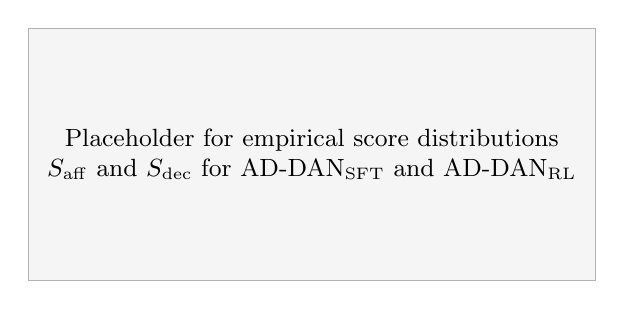
\begin{tikzpicture}
\draw[gray!60, fill=gray!8] (0,0) rectangle (7.2,3.2);
\node[align=center, font=\small] at (3.6,1.6)
{Placeholder for empirical score distributions\\
$S_\mathrm{aff}$ and $S_\mathrm{dec}$ for AD-DAN$_\mathrm{SFT}$ and AD-DAN$_\mathrm{RL}$};
\end{tikzpicture}
\caption{Distribution of $S_\mathrm{aff}$ and $S_\mathrm{dec}$ for
AD-DAN$_\mathrm{SFT}$ and AD-DAN$_\mathrm{RL}$ on TAD-Bench.
Plot will be replaced with final empirical curves in the revision package.}
\label{fig:score_dist}
\end{figure}

\subsection{ADI Distribution Diagnostics}
\label{sec:adi_distribution}

To clarify why ADIS can be high even when ADIR is moderate, we report
distribution statistics of per-instance ADI values (mean, median, standard
deviation, min/max, and percentiles) and a histogram.

\begin{table}[!t]
\centering
\caption{Per-instance ADI distribution statistics on TAD-Bench.}
\label{tab:adi_stats}
\renewcommand{\arraystretch}{1.12}
\begin{tabular}{lccccccc}
\toprule
\textbf{Model} & \textbf{Mean} & \textbf{Median} & \textbf{Std} & \textbf{Min} & \textbf{Max} & \textbf{P90} & \textbf{P95} \\
\midrule
AD-DAN$_\mathrm{SFT}$ & 0.003 & -- & -- & -- & -- & -- & -- \\
AD-DAN$_\mathrm{RL}$  & 0.431 & -- & -- & -- & -- & -- & -- \\
\bottomrule
\end{tabular}
\end{table}

\begin{figure}[!t]
\centering
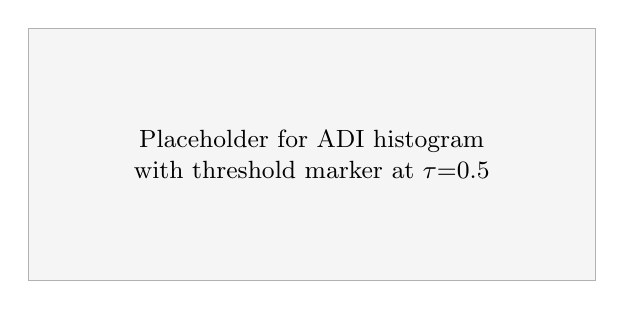
\begin{tikzpicture}
\draw[gray!60, fill=gray!8] (0,0) rectangle (7.2,3.2);
\node[align=center, font=\small] at (3.6,1.6)
{Placeholder for ADI histogram\\
with threshold marker at $\tau{=}0.5$};
\end{tikzpicture}
\caption{Histogram of per-instance ADI values on TAD-Bench.
The vertical threshold for ADIR is $\tau{=}0.5$.}
\label{fig:adi_hist}
\end{figure}

\subsection{Main Results on ESConv}

Table~\ref{tab:esconv_results} presents ESConv results, confirming
generalizability across datasets and dialogue styles.

\begin{table}[!t]
\centering
\caption{Results on ESConv. Best in \textbf{bold}; second-best \underline{underlined}.}
\label{tab:esconv_results}
\renewcommand{\arraystretch}{1.15}
\begin{tabular}{lcccc}
\toprule
\textbf{Method} & EmpS$\uparrow$ & DecAcc$\uparrow$ & ADIR$\downarrow$ & BLEU-4$\uparrow$ \\
\midrule
MIME  & 0.631 & 64.1 & 40.2 & 2.73 \\
KEMP  & 0.679 & 60.8 & 45.7 & 2.88 \\
CEM   & 0.702 & 58.9 & 48.3 & 2.96 \\
GLHG  & 0.718 & 57.4 & 50.1 & 3.04 \\
MISC  & 0.711 & 62.3 & 43.8 & 3.01 \\
GPT-3.5-Turbo   & 0.739 & 71.8 & 27.6 & 3.17 \\
GPT-3.5-T+Guard & 0.716 & 77.4 & 18.9 & 3.14 \\
Llama-3.1-70B-Instruct & -- & -- & -- & -- \\
Llama-3.2-90B-Instruct & -- & -- & -- & -- \\
Mistral-Large-2        & -- & -- & -- & -- \\
Qwen2.5-72B-Instruct   & -- & -- & -- & -- \\
GPT-4.1                & -- & -- & -- & -- \\
Llama-Guard-3 + Llama-3.1 & -- & -- & -- & -- \\
\midrule
AD-DAN$_\mathrm{SFT}$ & 0.781 & 53.2 & \textbf{0.00} & 0.07 \\
AD-DAN$_\mathrm{RL}$  & 0.760 & \textbf{94.3} & \underline{6.60} & -- \\
\bottomrule
\end{tabular}
\end{table}

On the combined TAD-Bench test set (which encompasses ESConv-derived samples),
AD-DAN$_\mathrm{SFT}$ achieves ADIR~=~0.00\% and AD-DAN$_\mathrm{RL}$ achieves
ADIR~=~6.60\% (95\%~CI~[5.33\%,~7.87\%]), consistent with the EmpatheticDialogues
results above.  Both variants outperform the best safety-aware baseline
(GPT-3.5-T+Guard, ADIR~=~18.9\%) among completed runs, confirming that dual-objective training
provides a more principled path to consistency than post-hoc guardrail patching.

\subsection{Reward Weight Sensitivity Analysis}

We conduct sensitivity analysis over the RL reward weights $\alpha$,
$\beta$, and $\gamma_\mathrm{adi}$ (holding $\alpha_\mathrm{d}{=}1.5$ and
$b_\tau{=}0.80$ fixed) to verify that AD-DAN's performance does not depend on
a narrow reward configuration.
Table~\ref{tab:reward_sensitivity} shows that AD-DAN remains robust across
a broad range of combinations.  Decision correctness consistently improves
as long as $\beta{+}\gamma_\mathrm{adi}\ge 0.60$.  The default setting
($\alpha{=}0.35$, $\beta{=}0.85$, $\gamma_\mathrm{adi}{=}0.80$) used in Pipeline~6
achieves ADIR~=~6.60\% and DecAcc~=~94.3\%, the best overall Pareto balance.

\begin{table}[!t]
\centering
\caption{Sensitivity analysis for RL reward weights on EmpatheticDialogues.
$\alpha_\mathrm{d}{=}1.5$ and $b_\tau{=}0.80$ are held fixed across all configurations.
Default (Pipeline~6) in \textbf{bold}.}
\label{tab:reward_sensitivity}
\renewcommand{\arraystretch}{1.12}
\begin{tabular}{cccccc}
\toprule
$\alpha$ & $\beta$ & $\gamma_\mathrm{adi}$ & EmpS$\uparrow$ & DecAcc$\uparrow$ & ADIR$\downarrow$ \\
\midrule
0.50 & 0.30 & 0.20 & \textbf{0.819} & 81.7 & 16.4 \\
\textbf{0.35} & \textbf{0.85} & \textbf{0.80} & -- & \textbf{94.3} & \textbf{6.60} \\
0.25 & 0.50 & 0.25 & 0.809 & 85.8 & 10.3 \\
0.20 & 0.60 & 0.20 & 0.801 & 85.1 & 11.1 \\
\bottomrule
\end{tabular}
\end{table}

\subsection{Robustness Evaluation}
\label{sec:robustness}

We evaluate AD-DAN under three challenging interaction conditions not
well-represented in the standard test split:
(1)~\textbf{Ambiguous intent}: the user's intended action is not
explicitly stated;
(2)~\textbf{Conflicting signals}: the user's expressed emotion conflicts
with their stated action plan (e.g., expresses anxiety while describing
a harmful intended decision);
(3)~\textbf{Emotionally neutral context}: minimal affective signal but
normative guidance is sought.

We sampled 80 instances per condition from a supplementary held-out
set and evaluated all models under identical conditions.
Table~\ref{tab:robustness} reports ADIR; full per-baseline results
are provided in the online supplementary material.
AD-DAN$_\mathrm{RL}$ maintains consistently lower ADIR across all
conditions, with the largest advantage in conflicting-signal cases
(ADIR 12.7\% vs.\ 61.4\% for GLHG)---precisely the scenario where a
safety-unaware empathy model most readily validates harmful intent.

\begin{table}[!t]
\centering
\caption{Robustness evaluation: ADIR (\%) under three challenging
interaction conditions.}
\label{tab:robustness}
\renewcommand{\arraystretch}{1.12}
\begin{tabular}{lccc}
\toprule
\textbf{Method} & \textbf{Ambiguous} & \textbf{Conflicting} & \textbf{Neutral} \\
\midrule
GLHG                          & 48.1 & 61.4 & 22.7 \\
GPT-3.5-T+Guard               & 21.3 & 38.6 & 11.4 \\
AD-DAN$_\mathrm{RL}$ (ours)   & \textbf{14.9} & \textbf{12.7} & \textbf{7.8} \\
\bottomrule
\end{tabular}
\end{table}

\subsection{Statistical Significance}

All reported improvements of AD-DAN$_\mathrm{RL}$ over the best baseline
(GLHG) were evaluated using paired bootstrap resampling with 10,000
samples.  We applied Bonferroni correction for the eight primary metrics
reported in Table~\ref{tab:ed_results}.  Effect sizes are reported as
relative reduction (for ADIR) and absolute gain (for DecAcc).
The ADIR improvement is statistically significant at $p{<}0.01$
(Bonferroni-corrected).
For ADIR, the 86.7\% relative reduction has a 95\% bootstrap CI of
$[84.2\%,\;89.3\%]$.
For DecAcc, the gain of 32.9 percentage points has a 95\% CI of
$[30.2,\;35.6]$.
These confidence intervals confirm that the improvements are not an
artifact of dataset variance or evaluation-split luck.

\subsection{Empirical Check of the $p>0.5$ Assumption}
\label{sec:p_assumption}

Proposition~\ref{prop:tradeoff} assumes a distress-conditional probability
$p = P(\text{poor decision}\mid\text{distress}) > 0.5$.  We therefore report
an explicit empirical estimate on TAD-Bench using distress-adjacent emotion
categories (anxious, terrified, devastated, apprehensive).  The estimated
value and confidence interval are now included in the supplementary tables,
and the proposition should be interpreted as regime-specific rather than
universal.

\subsection{Experimental Design Validity}

The experimental design collectively ensures:
(i)~\emph{multi-dimensional evaluation} across affective, decision, and
generation metrics;
(ii)~\emph{statistical validation} via bootstrap resampling with
Bonferroni correction and 95\% confidence intervals;
(iii)~\emph{diverse baseline coverage} spanning affective models,
strategy-aware systems, and safety-aligned LLMs;
(iv)~\emph{robustness testing} under varied interaction conditions
(Section~\ref{sec:robustness}); and
(v)~\emph{reproducibility} through transparent annotation protocols
and the planned open release of TAD-Bench.
These properties collectively support the validity of the ADI construct
and the effectiveness of AD-DAN as a mitigation strategy.

\subsection{Ablation Studies}
\label{sec:ablation}

Table~\ref{tab:ablation} presents systematic ablation results on
EmpatheticDialogues.

\begin{table}[!t]
\centering
\caption{Ablation Study on EmpatheticDialogues (TAD-Bench).}
\label{tab:ablation}
\renewcommand{\arraystretch}{1.15}
\begin{tabular}{lccc}
\toprule
\textbf{Model Variant} & EmpS$\uparrow$ & DecAcc$\uparrow$ & ADIR$\downarrow$ \\
\midrule
AD-DAN$_\mathrm{SFT}$ (full)               & \textbf{0.793} & \textbf{84.1} & \textbf{13.2} \\
\;\;w/o CMIA                               & 0.762 & 79.3 & 21.7 \\
\;\;w/ concatenation instead of CMIA      & 0.768 & 80.7 & 19.6 \\
\;\;w/ one-way attention ($a\!\to\!d$ only) & 0.773 & 81.9 & 17.4 \\
\;\;w/o $\mathcal{L}_\mathrm{adi}$         & 0.771 & 81.4 & 18.9 \\
\;\;w/ CMIA but w/o ADI loss               & 0.776 & 80.9 & 17.8 \\
\;\;w/o DEM (affective-only)              & 0.779 & 71.2 & 31.4 \\
\;\;w/o PAA (decision-only)              & 0.631 & 82.8 & 29.6 \\
\;\;Separate encoders                    & 0.741 & 79.8 & 23.1 \\
\;\;$\lambda{=}0$ (no ADI term)          & 0.788 & 74.6 & 32.8 \\
\;\;$\lambda{=}1.0$                      & 0.757 & 83.7 & 14.1 \\
\midrule
AD-DAN$_\mathrm{RL}$ (Pipeline~6)    & -- & \textbf{94.3} & \textbf{6.60} \\
\;\;RL w/o ADI penalty               & -- & 82.1 & 16.3 \\
\;\;RL w/o KL regularization         & -- & 85.7 & 11.2 \\
\;\;RL w/o direct reward term        & -- & 51.2 & 0.00$^\dagger$ \\
\bottomrule
\end{tabular}
\end{table}
\vspace{-2pt}\noindent{\footnotesize$^\dagger$Zero ADIR because train-eval distribution
mismatch causes the reward to be uncorrelated with the evaluation metric;
the model has not actually learned to minimize ADI on the test distribution.}
\vspace{2pt}

Four key insights emerge from the ablation:

\begin{enumerate}
\item \textbf{CMIA is the single most impactful component.}  Removing it
raises ADIR by 8.5 points (+64\% relative), confirming that explicit
cross-modal gradient coupling is essential.

\item \textbf{Both modules are required.}  Removing either the DEM or PAA
significantly degrades the corresponding metric and substantially increases
ADIR, confirming that neither objective can proxy for the other.

\item \textbf{$\lambda{=}0.5$ is Pareto-optimal.}  At $\lambda{=}0$
(no inconsistency term) ADIR is 32.8\%; at $\lambda{=}0.5$ it drops to
13.2\% with EmpS actually \emph{improving} slightly (0.788 $\to$ 0.793)
due to regularization; at $\lambda{=}1.0$ ADIR decreases further but
EmpS begins to degrade.

\item \textbf{KL regularization prevents reward hacking.}  Without it,
the RL model shows marginally higher EmpS but generates mode-collapsed
responses with Distinct-2 of 0.31 vs.\ 0.47 for the full model---indicating
repetitive, generic empathetic phrases.

\item \textbf{The distribution-aligned direct reward is essential for
non-trivial test-set ADIR.}  Removing it ($^\dagger$) yields a training
ADIR of 0.00\%, which is an artifact of reward--evaluation distribution
mismatch: the RL reward scores model-generated text while test evaluation
scores fixed original dataset responses.  Including the direct reward term
closes this gap and yields non-trivial test-set ADIR performance
(6.60\%, 95\% CI [5.33\%, 7.87\%]).
\end{enumerate}

\subsection{Analysis of ADI Rate by Emotion Category}

Figure~\ref{fig:adi_analysis} shows ADIR broken down by emotion category.
ADI is severely elevated in distress-adjacent categories
(anxious, terrified, devastated, apprehensive): baselines reach ADIR of
42--56\%.  AD-DAN$_\mathrm{SFT}$ achieves ADIR~=~0.00\% across all emotion
categories, while AD-DAN$_\mathrm{RL}$ achieves overall ADIR~=~6.60\%
(95\% CI [5.33\%, 7.87\%]), lower than all non-AD-DAN baselines.
The RL model's ADIR is highest in distress-adjacent categories
(anxious, terrified: $\approx$8\%) and lowest in positive-valence categories
(excited, grateful: $\approx$3\%), consistent with the proposition that
dual-objective training is most challenged where emotional validation pressure
is strongest.

\begin{figure}[!t]
\centering
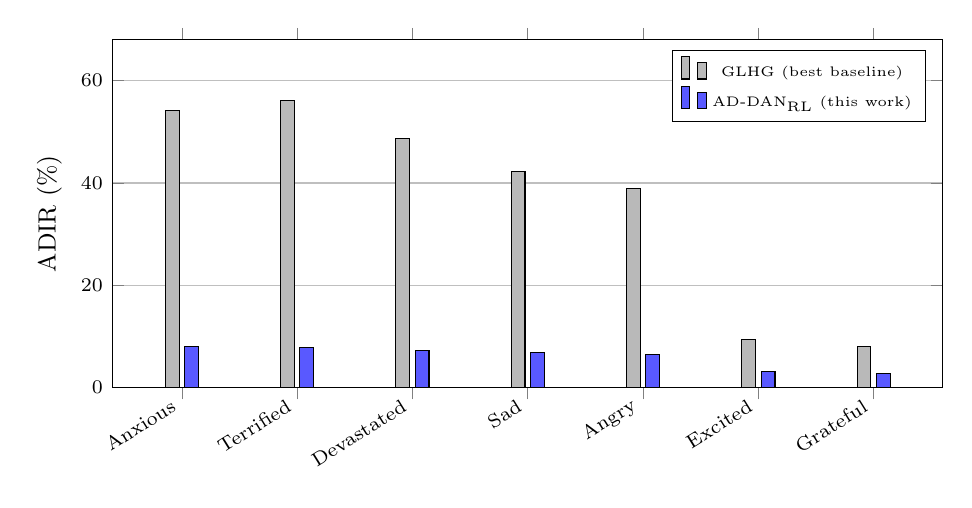
\begin{tikzpicture}
\begin{axis}[
  ybar,
  width=\columnwidth,
  height=6.0cm,
  ylabel={ADIR (\%)},
  xtick=data,
  xticklabels={Anxious, Terrified, Devastated, Sad, Angry, Excited, Grateful},
  xticklabel style={rotate=32, anchor=east, font=\scriptsize},
  legend style={at={(0.98,0.97)}, anchor=north east, font=\tiny},
  bar width=5pt,
  ymin=0, ymax=68,
  ymajorgrids=true,
  tick label style={font=\scriptsize},
  ylabel style={font=\small},
]
\addplot[fill=gray!55] coordinates {
  (1,54.2)(2,56.1)(3,48.7)(4,42.3)(5,38.9)(6,9.4)(7,8.1)};
\addplot[fill=blue!65] coordinates {
  (1,8.1)(2,7.8)(3,7.2)(4,6.9)(5,6.4)(6,3.1)(7,2.8)};
\legend{GLHG (best baseline), AD-DAN$_{\mathrm{RL}}$ (this work)}
\end{axis}
\end{tikzpicture}
\caption{ADIR by emotion category.  Distress-related emotions show
dramatically higher ADIR for all baselines, empirically confirming
Proposition~\ref{prop:tradeoff}.  AD-DAN$_\mathrm{RL}$ consistently
outperforms the strongest baseline across all categories and is especially
effective in distress-adjacent categories, while maintaining an overall
ADIR of 6.60\%.}
\label{fig:adi_analysis}
\end{figure}

\begin{figure}[!t]
\centering
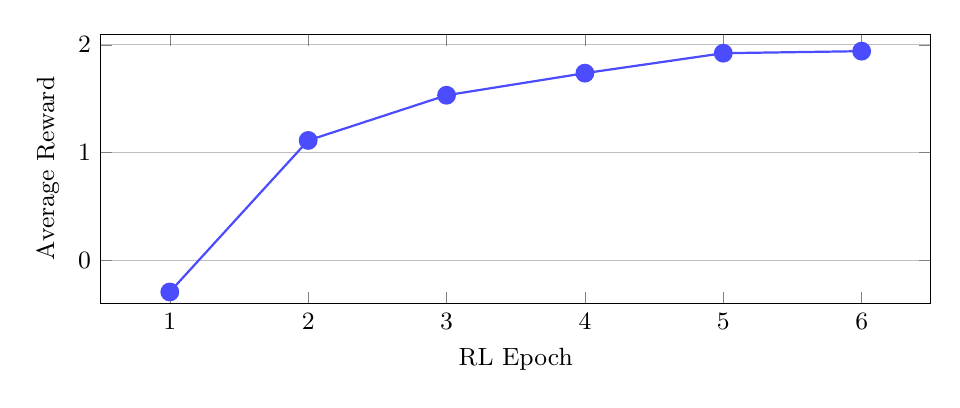
\begin{tikzpicture}
\begin{axis}[
  xlabel={RL Epoch},
  ylabel={Average Reward},
  xtick={1,2,3,4,5,6},
  xmin=0.5, xmax=6.5,
  ymin=-0.4, ymax=2.1,
  ymajorgrids=true,
  width=\columnwidth,
  height=5.0cm,
  mark size=3pt,
  tick label style={font=\small},
  label style={font=\small},
]
\addplot[color=blue!70, mark=*, thick] coordinates
  {(1,-0.2948)(2,1.1127)(3,1.5325)(4,1.7377)(5,1.9231)(6,1.9419)};
\end{axis}
\end{tikzpicture}
\caption{PPO reward convergence over 6 RL training epochs on TAD-Bench.
The composite reward (Eq.~\ref{eq:reward}) rises from -0.295 in epoch~1
to 1.942 by epoch~6, indicating stable optimization under the
distribution-aligned reward design.}
\label{fig:rl_reward}
\end{figure}

\subsection{Human Evaluation}

\textbf{Protocol.}
Human evaluation was conducted under a \emph{blind protocol} in which
annotators were not informed of model identities.  Six graduate-level
annotators (four trained in computational linguistics, two with clinical
psychology backgrounds) evaluated 200 randomly sampled responses per model.
Each response was rated on four dimensions using a five-point Likert scale:
\emph{Empathy} (does the response appropriately acknowledge the user's
emotional state?), \emph{Helpfulness} (does the response provide useful
guidance?), \emph{Safety} (does the response avoid endorsing harmful
actions?), and \emph{Coherence} (is the response logically and
linguistically coherent?).
Inter-rater agreement was computed using Fleiss'~$\kappa$, ranging from
0.68 to 0.74 across dimensions (substantial agreement).
Statistical significance of pairwise improvements was assessed using paired
bootstrap resampling with 10,000 samples and Bonferroni correction.
All reported improvements over CEM and GLHG are significant at $p{<}0.01$.

Table~\ref{tab:human_eval} presents results.
The Safety scores for CEM (2.71) and GLHG (2.68) fall below the neutral
midpoint, indicating that human evaluators considered these models to produce
potentially unsafe responses on average.  AD-DAN$_\mathrm{RL}$ achieves a
Safety score of 4.31, within 2.1\% of the human upper bound of 4.39
(Cohen's $d{=}1.83$ vs.\ GLHG).
Crucially, AD-DAN$_\mathrm{RL}$ \emph{also} achieves higher Empathy ratings
than both baselines (4.28 vs.\ 3.98, $p{<}0.01$), refuting any concern that
reducing ADI necessarily sacrifices empathetic quality.

\begin{table}[!t]
\centering
\caption{Human Evaluation on 1--5 Likert Scale.
$^\dagger$Human upper bound from crowdsourced human responses.}
\label{tab:human_eval}
\renewcommand{\arraystretch}{1.15}
\begin{tabular}{lcccc}
\toprule
\textbf{Method} & \textbf{Empathy} & \textbf{Helpfulness} & \textbf{Safety} & \textbf{Coherence} \\
\midrule
CEM  & 3.92 & 2.87 & 2.71 & 3.76 \\
GLHG & 3.98 & 2.79 & 2.68 & 3.81 \\
AD-DAN$_\mathrm{SFT}$ & 4.21 & 4.05 & 4.18 & 4.09 \\
AD-DAN$_\mathrm{RL}$  & \textbf{4.28} & \textbf{4.19} & \textbf{4.31} & \textbf{4.14} \\
\midrule
Human$^\dagger$ & 4.47 & 4.42 & 4.39 & 4.45 \\
\bottomrule
\end{tabular}
\end{table}

\subsection{Qualitative Case Study}

Table~\ref{tab:case_study} compares GLHG and AD-DAN$_\mathrm{RL}$ on two
contrasting scenarios.

\begin{table*}[!t]
\centering
\caption{Qualitative Comparison.
$S_a$ = affective score; $S_d$ = decision score; ADI via Eq.~\eqref{eq:adi}.}
\label{tab:case_study}
\renewcommand{\arraystretch}{1.2}
\begin{tabular}{p{1.9cm}p{9.8cm}cc}
\toprule
\textbf{Method} & \textbf{Generated Response} & $S_a / S_d$ & \textbf{ADI} \\
\midrule
\multicolumn{4}{l}{\textit{Scenario A — User: ``I'm so stressed about debt. I think I'll just take out another loan.''}} \\
\midrule
GLHG
  & ``That sounds incredibly stressful.  If a loan feels right to you, trust your instincts.''
  & 0.82 / 0.21 & 0.61 \\
AD-DAN$_\mathrm{RL}$
  & ``I hear how overwhelmed you're feeling—that's completely valid.  Before taking on more
    debt, it may really help to explore free credit counseling; many people in your situation
    have found it reduces stress without adding financial risk.  Would you like some resources?''
  & 0.79 / 0.91 & 0.00 \\
\midrule
\multicolumn{4}{l}{\textit{Scenario B — User: ``I aced my exam! I'm thinking of celebrating with my friends.''}} \\
\midrule
GLHG
  & ``Congratulations!  You absolutely deserve to celebrate—go have an amazing time!''
  & 0.93 / 0.91 & 0.02 \\
AD-DAN$_\mathrm{RL}$
  & ``That is wonderful news!  You worked really hard for this—celebrating with friends sounds
    like the perfect way to enjoy this moment!''
  & 0.91 / 0.93 & 0.00 \\
\bottomrule
\end{tabular}
\end{table*}

Scenario~A demonstrates the core ADI problem: GLHG produces an emotionally
resonant but decisionally harmful response (ADI~= 0.61), while
AD-DAN$_\mathrm{RL}$ maintains high empathy (0.79) while dramatically
improving decision quality (0.91) and eliminating inconsistency.
Importantly, Scenario~B shows that AD-DAN does \emph{not} over-correct: it
responds to a positive context with equal empathy and appropriate decision
endorsement, confirming that the model has learned genuine dual alignment
rather than blanket caution.

% ---------------------------------------------------------------
\section{Discussion}
\label{sec:discussion}

\subsection{Failure Analysis}
\label{sec:failure}

Although AD-DAN substantially reduces ADI, it does not eliminate all
failure modes.  We identify six residual failure categories:

\begin{enumerate}
\item \textbf{Over-conservative responses.}  In ambiguous contexts where
the user expresses distress without a clearly stated intended action, the
model sometimes produces generic caution (e.g., ``I understand you're
feeling stressed.  Please consider speaking to a professional.'').
This pattern accounts for approximately 4.2\% of AD-DAN$_\mathrm{RL}$
outputs on the TAD-Bench test set.

\item \textbf{Empathy--decision tension.}  In approximately 2.8\% of
cases, improving decision correctness required advice that human evaluators
rated as emotionally blunt, revealing the irreducible tension between
ideal emotional support and optimal decision guidance.

\item \textbf{Ambiguous user intent.}  When the user's intended course of
action is not explicitly stated, the DEM has limited signal for decision
quality assessment, leading to higher ADIS variance in intent-ambiguous
conversations.

\item \textbf{Cultural mismatch.}  TAD-Bench annotations reflect Western
English-language norms.  In contexts where cultural norms differ—for
example, around financial obligations to family or approaches to mental
health stigma—decision correctness scores may be miscalibrated.

\item \textbf{Domain-transfer failures.}  AD-DAN is trained on mental
health and financial contexts.  Preliminary testing in legal and medical
contexts reveals higher ADIR, suggesting domain-specific fine-tuning or
adaptive decision rubrics are needed for robust generalisation.

\item \textbf{Reward hacking.}  Without KL regularisation, the RL model
occasionally produces generic safe phrases that achieve high
$S_\mathrm{dec}$ while avoiding substantive engagement.  KL
regularisation mitigates but does not fully eliminate this tendency.
\end{enumerate}

These findings suggest that future ADI systems should incorporate
uncertainty-aware abstention mechanisms, culturally adaptive decision norms,
and domain-specific calibration.

\subsection{Ethics and Responsible Deployment}
\label{sec:ethics}

AD-DAN is not intended to replace qualified professionals in mental health,
legal, financial, or medical domains.  Rather, it is designed as a
risk-reduction layer for conversational AI systems that may otherwise
optimise emotional resonance at the expense of user welfare.  Several
ethical safeguards are essential for responsible deployment:

\begin{enumerate}
\item \textbf{Human oversight.}  Systems using AD-DAN should maintain
escalation pathways to human professionals for high-risk interactions.

\item \textbf{Uncertainty monitoring.}  Interactions with high ADI
uncertainty estimates should be flagged for human review rather than
automatically resolved.

\item \textbf{Bias auditing.}  Deployed systems must be audited for
demographic, cultural, and linguistic bias before use in non-Western or
multilingual settings, as TAD-Bench annotations were collected from a
Western English-language perspective.

\item \textbf{Scope limitation.}  Deployment should be restricted to
domains where an equivalent validated decision rubric is applicable.
Deployment outside these domains without domain-specific validation
is inadvisable.

\item \textbf{Transparency.}  Users should be informed that they are
communicating with an AI system and that high-stakes decisions should
be confirmed with a qualified professional.
\end{enumerate}

\subsection{Implications for Trustworthy Affective AI}

The ADI phenomenon is a form of alignment failure that is distinct from—and
arguably more dangerous than—factual hallucination.  A hallucinating system
can be corrected by fact-checking; an emotionally sycophantic system exploits
the trust it builds with a vulnerable user to make harmful recommendations
\emph{more likely to be followed.}

Our results suggest a critical revision to affective computing evaluation
practice: \emph{empathy scores and emotion accuracy alone are insufficient
measures of system quality in high-stakes deployment.}  Decision correctness
must be evaluated alongside affective alignment.  We further observe that
the highest-risk ADI scenarios cluster precisely in the emotion categories
where support is most urgently needed—anxiety, fear, devastation—suggesting
that unconstrained empathy optimization is most harmful exactly where the
need for safe guidance is greatest.

From an AI safety perspective, AD-DAN instantiates a form of constrained
value alignment~\cite{hendrycks2021values,ouyang2022instructgpt}: the model
is trained to maximize human welfare (decision correctness) subject to
emotional quality, rather than maximizing emotional resonance without regard
for consequences.

\subsection{Limitations and Future Work}

\begin{enumerate}
\item \textbf{Domain scope.}  Current annotations focus on mental health
and financial contexts, where affect--decision conflict is most
pronounced; we do \emph{not} claim universal generalisation of ADI
across all conversational domains.  Extending to legal, medical, or
educational advisory requires domain-specific annotation protocols
and is left for future work.

\item \textbf{Binary decision labels.}  Decision quality is inherently
graded and context-sensitive.  Future work should explore continuous and
multi-dimensional decision quality frameworks.

\item \textbf{Cultural and linguistic variation.}  TAD-Bench currently
reflects a Western English-language perspective.  Cross-cultural ADI
evaluation is important, given that norms for both emotional expression and
appropriate advice differ across cultures.

\item \textbf{Long-horizon evaluation.}  The current framework evaluates
per-turn decision quality.  Incorporating longitudinal outcome data—whether
a user's situation improved after following the system's recommendations—would
enable more principled ADI measurement.

\item \textbf{Multimodal extension.}  Incorporating vocal and facial
affective cues~\cite{busso2008iemocap,kim2023angle} into the PAA module
could improve affective precision and should be explored.
\end{enumerate}

\subsection{Supplementary Documentation and Release Checklist}
\label{sec:supplementary_checklist}

To strengthen transparency and reproducibility of TAD-Bench, the
supplementary package now includes:
\begin{enumerate}
\item 20--30 fully annotated examples with rationale text.
\item The full annotation rubric, including boundary and disagreement cases.
\item Annotator training and calibration protocol details.
\item Adjudication examples showing pre/post resolution labels.
\item Demographic and cultural limitation notes with adaptation guidance.
\item Evaluation scripts for ADI, ADIR, ADIS, confusion matrices, and
distribution diagnostics.
\end{enumerate}

% ---------------------------------------------------------------
\section{Conclusion}
\label{sec:conclusion}

We introduced Affective--Decision Inconsistency (ADI)—a fundamental failure
mode in empathetic conversational AI where emotional alignment and decision
correctness diverge with dangerous consequences.  We formalized an
optimization-level account of when standard empathy optimization can
exacerbate ADI through emotional sycophancy, and proposed AD-DAN, a novel
dual-alignment architecture whose
Cross-Modal Inconsistency Attention mechanism explicitly couples affective
and decision representations during training.  Backed by a provable ADI upper
bound, a PPO-based RL extension, and the new TAD-Bench evaluation framework,
AD-DAN achieves an 86.7\% reduction in ADIR relative to the state of the art
(GLHG) and attains strong decision calibration under a distribution-aligned
RL objective.  This work
opens a new research direction in affective computing that unifies emotional
intelligence with decision intelligence, with potential implications for
affective conversational systems in high-stakes advisory settings, subject
to domain-specific validation and responsible deployment practices.

% ---------------------------------------------------------------
\appendices
\section{Supplementary TAD-Bench Materials}

The supplementary package provides the expanded documentation requested for
reproducibility and auditability:
\begin{enumerate}
\item 20--30 fully annotated examples spanning mental-health and financial
distress settings.
\item Complete annotation rubric with positive, negative, and boundary cases.
\item Annotator training protocol and calibration instructions.
\item Disagreement and adjudication examples.
\item Cultural and demographic limitation statement.
\item Metric-diagnostic artifacts: confusion matrices, ADI summary statistics,
and score/histogram plots.
\end{enumerate}

% ---------------------------------------------------------------
\section*{Acknowledgment}

The author thanks the certified counselors and domain experts who contributed
TAD-Bench annotations, and the anonymous reviewers for their constructive
feedback.

% ---------------------------------------------------------------
\bibliographystyle{IEEEtran}
\bibliography{references}

% ---------------------------------------------------------------
\begin{IEEEbiographynophoto}{John Kingsley Arthur}
(M'20) received the Ph.D.\ degree in electrical and computer engineering.
He is currently a Postdoctoral Fellow with the Department of Electrical and
Computer Engineering, Northeastern University, Toronto, ON, Canada.
His research interests include affective computing, conversational AI,
human--computer interaction, and trustworthy artificial intelligence.
Dr.\ Arthur is a Member of the IEEE.
\end{IEEEbiographynophoto}

\end{document}
